\documentclass[12pt]{article}
\usepackage{fullpage}
\usepackage{enumerate}
\usepackage{graphicx}

\begin{document}
Guocui Gao, Shuyan Guo, Thomas Schaffner, Jayme Woogerd \\
\indent Comp 116 - Security \\
\indent November 4, 2014 \\
\indent Capture the Flag Writeup \\

\begin{enumerate}[1.]
\item \textbf{Just ask for it}: Directory traversal

\textbf{Location}: \texttt{http://67.23.79.113/flag.txt}

This flag was simple directory traversal: there is a 'flag.txt' file on the server, accessible to the public, which contains the first flag. We guessed likely file paths until we found it.\\

	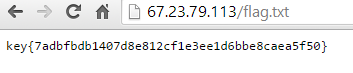
\includegraphics[scale=0.8]{images/flag1} \\

\item \textbf{Just ask for it with a catch -- packed refs}: Directory traversal

\textbf{Location}: \texttt{http://67.23.79.113/.git/packed-refs}

Similar to the first key, we used directory traversal to find the \texttt{.git} folder on the server. \\
In the \texttt{.git} folder, it is possible to download the \texttt{packed-refs} file: \\ \\

	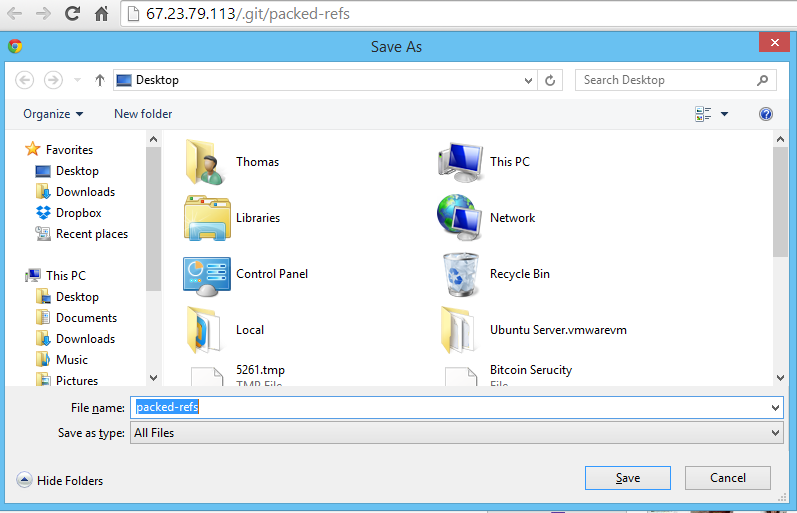
\includegraphics[scale=0.5]{images/flag2a} \\ \\

\newpage

We found the key at the bottom of the \texttt{packed-refs} file, among the real git references: \\

	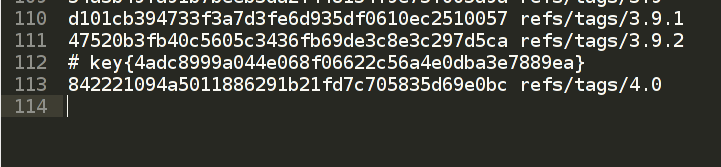
\includegraphics[scale=0.5]{images/flag2b} \\

\item \textbf{Analyze the binary}: Wireshark analysis of pcap file

\textbf{Location}: \texttt{fun.exe, paper.pdf}

We used the 'file' command in Linux to detect the real file type of \texttt{fun.exe}, which turned out to be a pcap file. \\

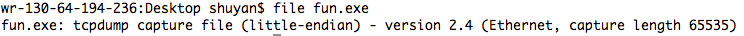
\includegraphics[scale=0.7]{images/flag3a} \\

Viewing the pcap file in Wireshark and following the TCP stream in it, we found a file called 'paper': \\

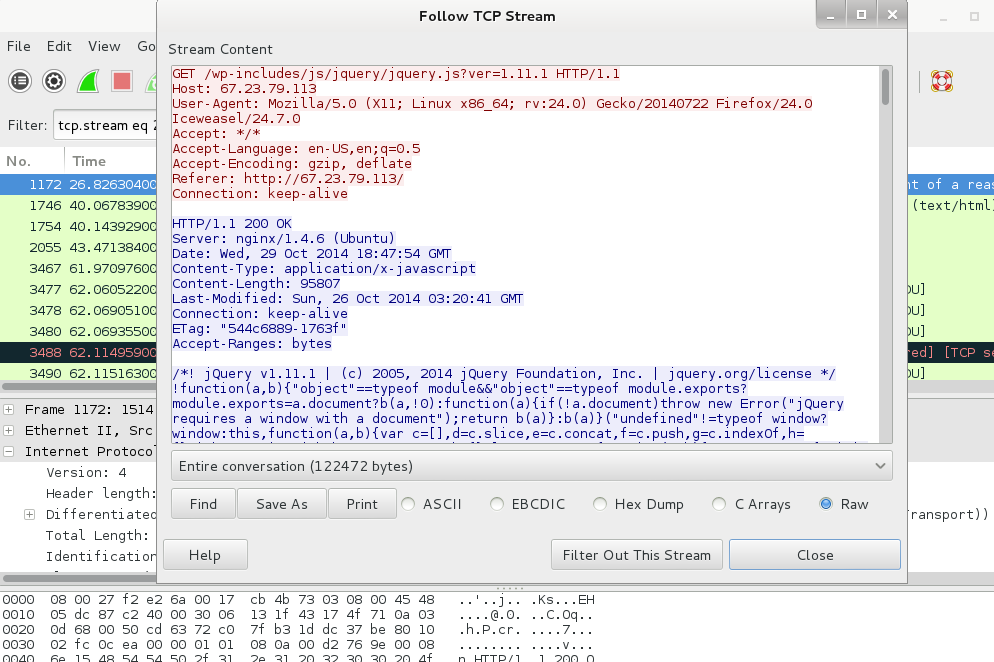
\includegraphics[scale=0.35]{images/flag3b} \\ \\

\newpage

We saved the TCP stream as \texttt{paper.pdf} and then opened the file to find the key:\\

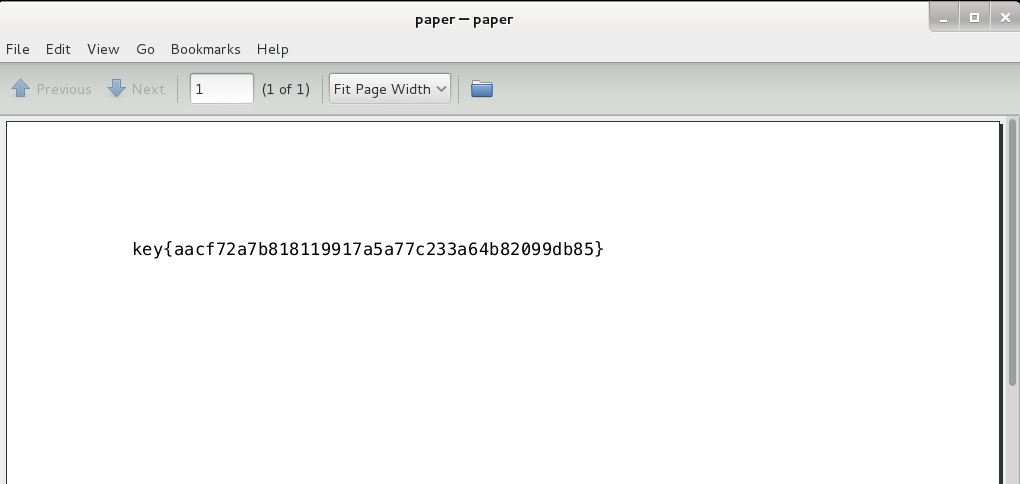
\includegraphics[scale=0.3]{images/flag3c} \\ \\

\item \textbf{I want to see MOAR on the board!}: Moar SQL injection:

\textbf{Location}: \texttt{http://67.23.79.113/board.php?id=1}

This was another SQL injection: clicking on any of the
posts on \texttt{board.php} navigated us to a page with
more details about that post. We noticed that when we did
this, the navigation bar changed -- adding the post id to the end of the URL (e.g. \texttt{id=1}). Changing this 
payload to \texttt{id=1 or true}, brought us to a special
post page with many MOAR memes...and the flag
buried in one of the posts.

By the time we got to this key, someone had injected a 
terrible script, which broke the browser. To actually find
the key, we had to use \texttt{curl} and then grep for the key:

\texttt{curl "http://67.23.79.113/board.php?id=1\%20or\%20true" | grep "key"} \\

\item \textbf{Look again, pay careful attention}: SQL injection via login credentials textbox

\textbf{Location}: \texttt{http://67.23.79.113/main.php}

Clicking on the 'Admin' link on \texttt{board.php} directs to a login page with
 input boxes for a username and password (\texttt{http://67.23.79.113/admin.php}). 
 To login, we used a simple SQL injection payload (a' or '1' = '1) in both 
 the username and password fields. Upon successful login, we got to what 
 looked like a 404 page; the flag was actually buried in the source: \\

  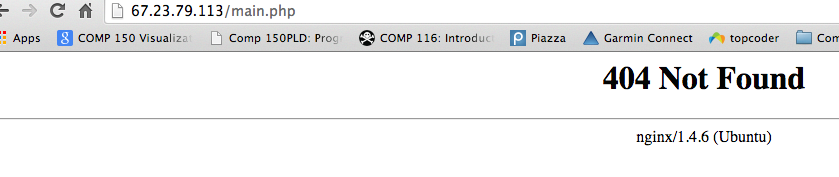
\includegraphics[scale=0.40]{images/flag5a} \\ \\
  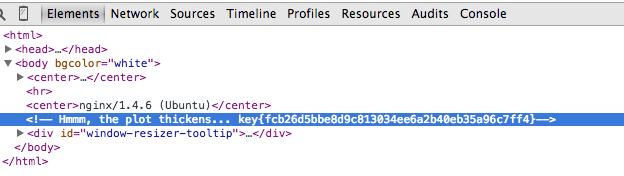
\includegraphics[scale=0.6]{images/flag5b}

\item \textbf{Look again, pay really careful attention}: Cookie tampering

\textbf{Location}: \texttt{http://67.23.79.113/main.php}

After logging into \texttt{http://67.23.79.113/main.php} via SQL injection, we viewed the site cookies via Chrome Developer Console:\\

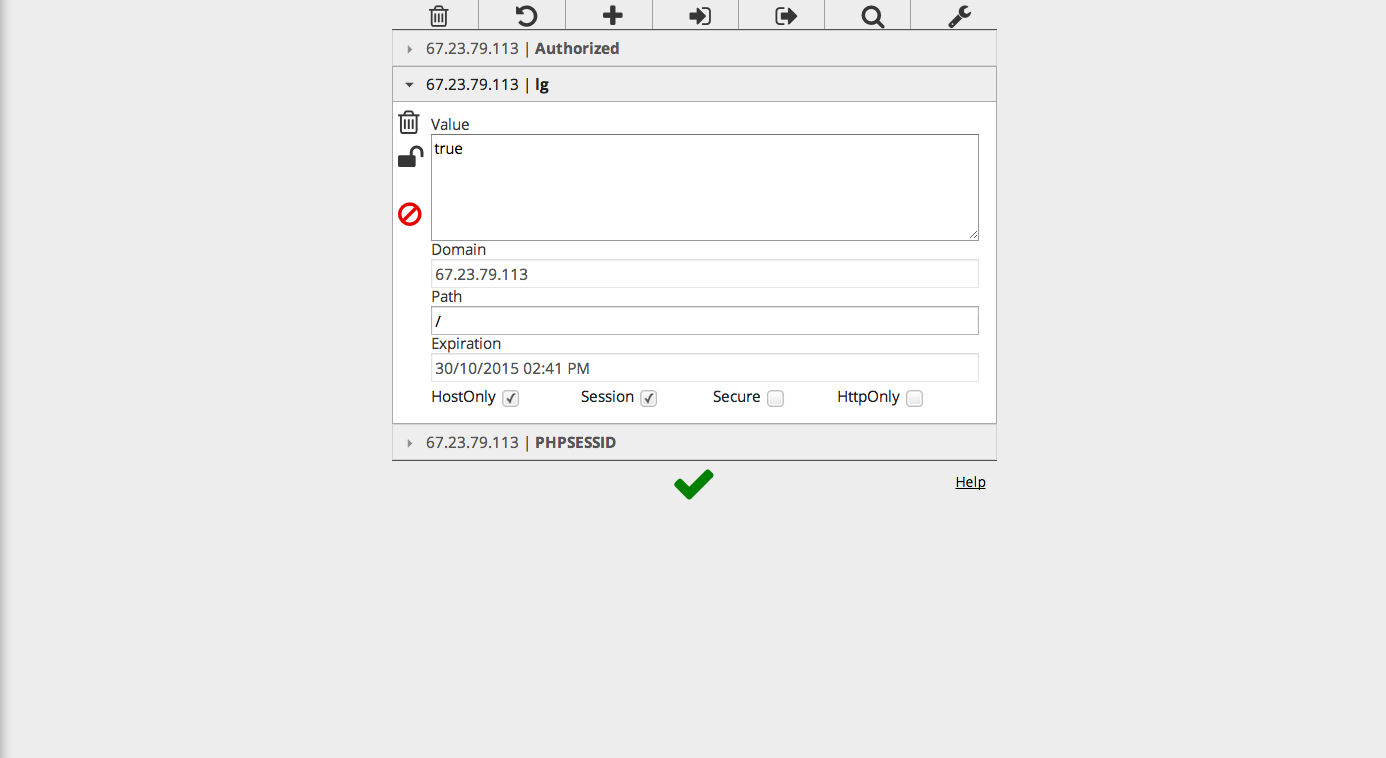
\includegraphics[scale=0.25]{images/flag6a} \\ \\

\newpage
Under the Resources tag, we found an item named 'lg' with value of 'false'. After changing the value to 'true' and reloading the web page, the key appeared:\\

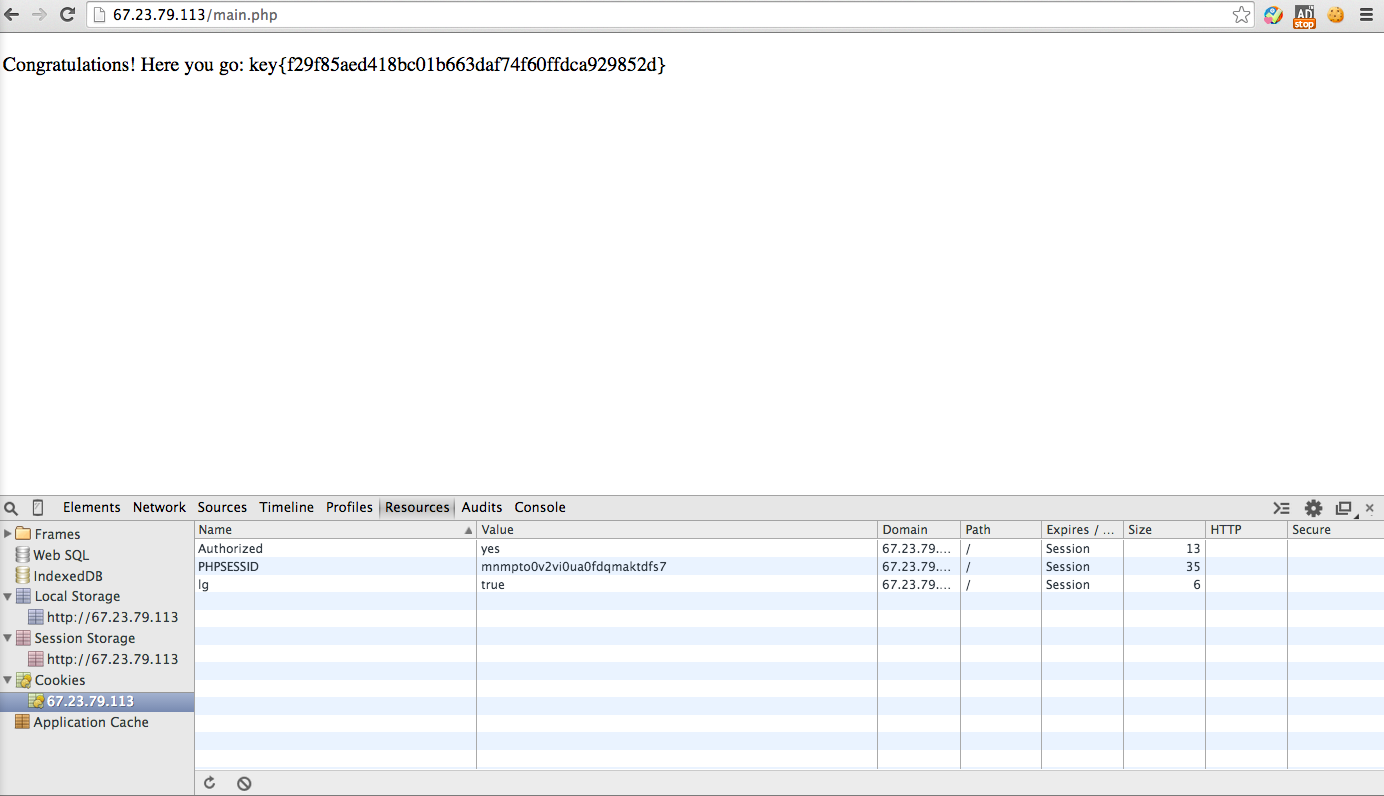
\includegraphics[scale=0.30]{images/flag6b} \\ \\

\item \textbf{Remember, you have to log out too!}: SQL injection, traversal

\textbf{Location}: \texttt{http://67.23.79.113/logout.php} 

First, we logged in to the 'Admin' page via the SQL injection described above in (5). Next, we simply navigated to \texttt{http://67.23.79.113/logout.php}: \\

  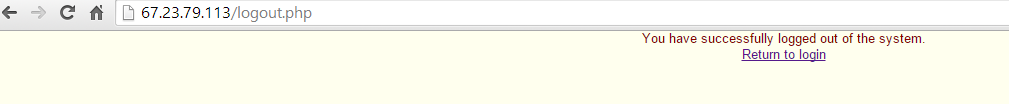
\includegraphics[scale=0.5]{images/flag7a} \\ \\

\newpage
 The key is not directly apparent, but we searched through the source and found the key at the bottom of the page: \\ 

  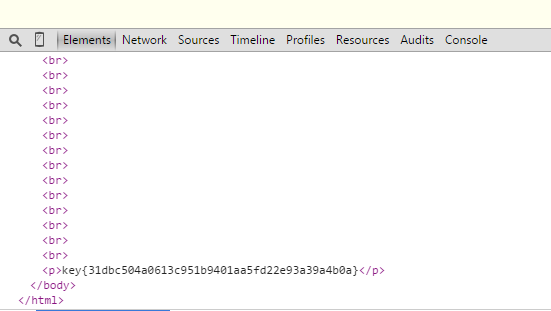
\includegraphics[scale=0.5]{images/flag7b} \\ \\

\item \textbf{Buried in the dump}: SQL injection

\textbf{Location}: \texttt{http://67.23.79.113/board.php}

We ran an automatic SQL injection tool in Kali called sqlmap on \texttt{board.php} and found that there existed five databases: \\

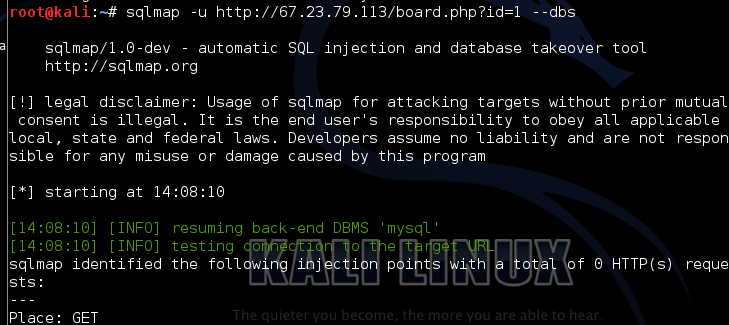
\includegraphics[scale=0.5]{images/flag8a} \\

One of them is called 'board' which contained a table called 'users': \\

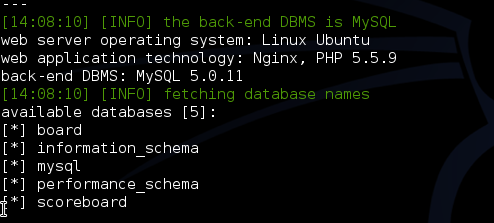
\includegraphics[scale=0.5]{images/flag8b} \\

Further extracting data from this table, we found the key disguised as a password for login 'lcontreras': \\

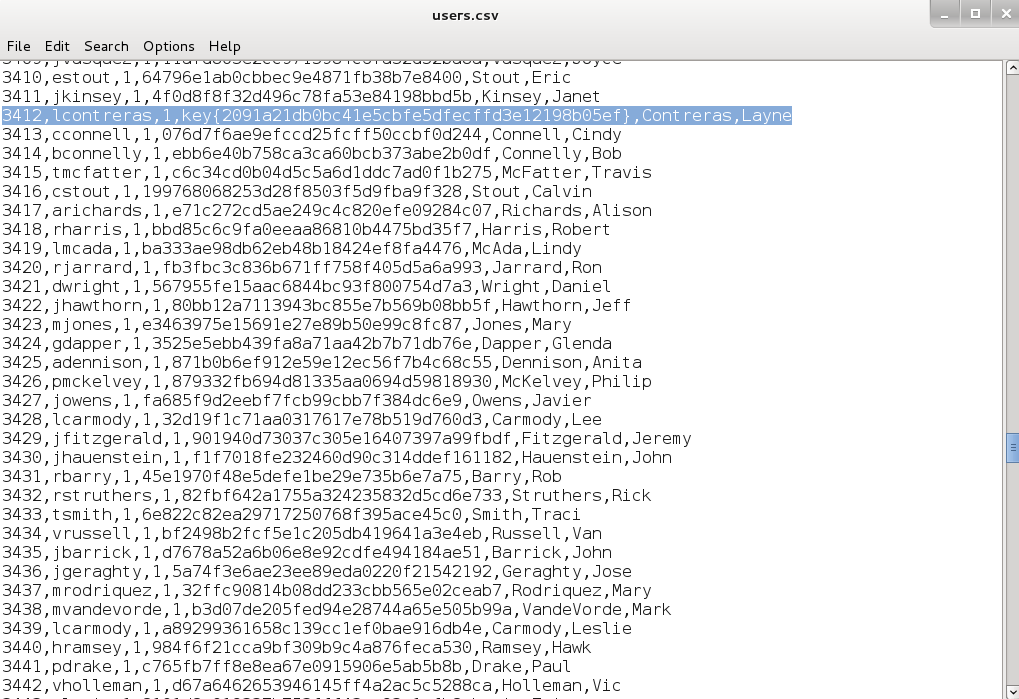
\includegraphics[scale=0.35]{images/flag8c} \\

\newpage

\item \textbf{All your base64 belong to us}: Base64 decoding

\textbf{Location}: \texttt{http://67.23.79.113/ngtnw}

From the hint, we guessed there existed a page named \texttt{ngtnw}. We went to \\ \texttt{http://67.23.79.113/ngtnw} and it appeared to be a game. After we played and lost the game, a dialog box prompted asking for name input. Upon submission, we checked the local storage of the web browser and found a value of the score we got followed by a string that seemed to be encoded in Base64: \\

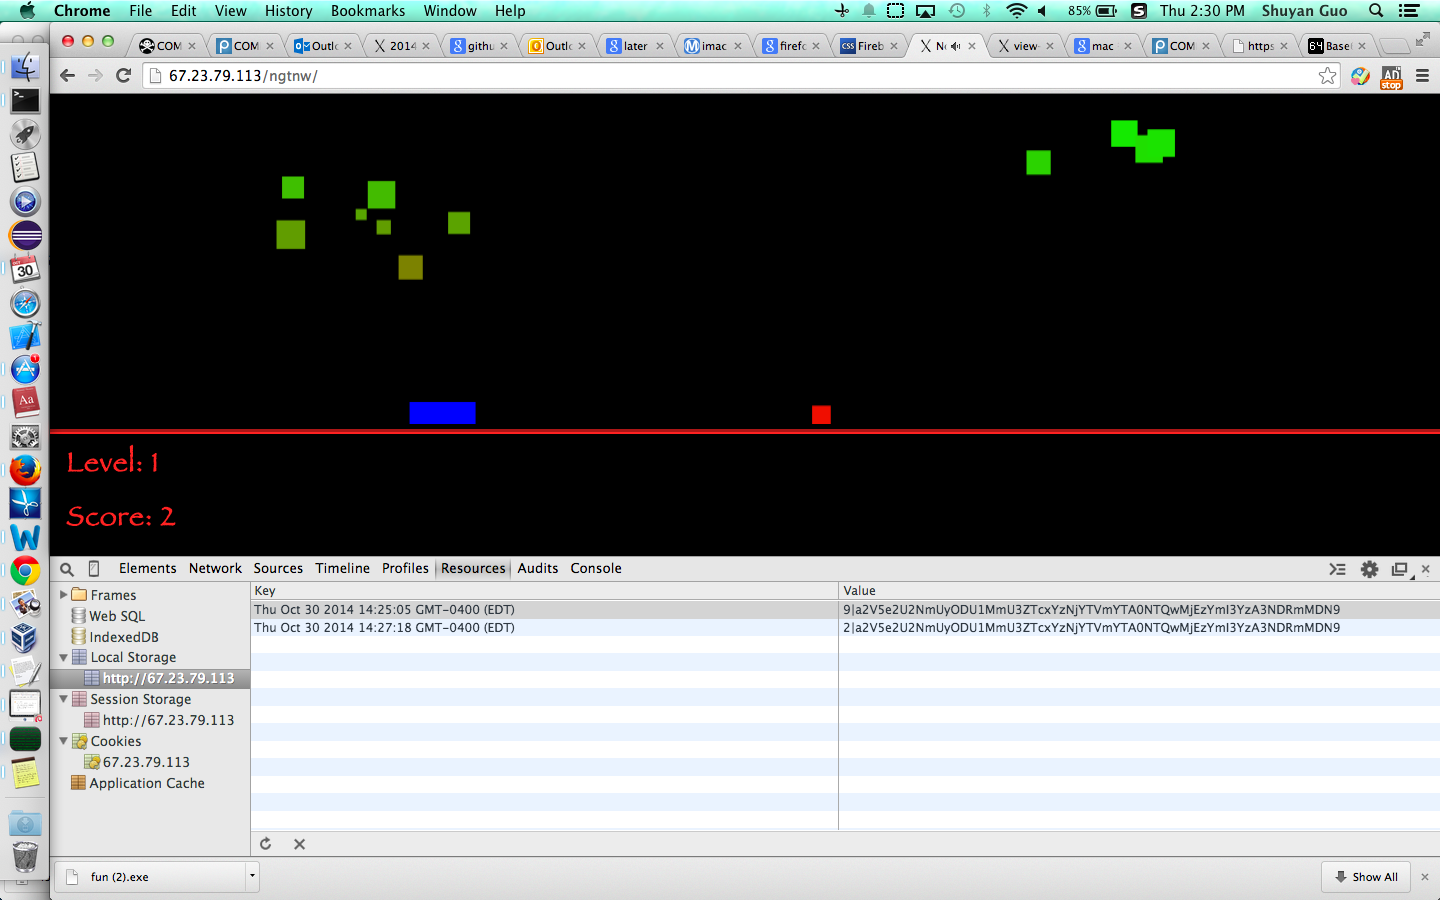
\includegraphics[scale=0.25]{images/flag9a} \\

Decoding the string with an online Base64 decoder tool, we found the key: \\

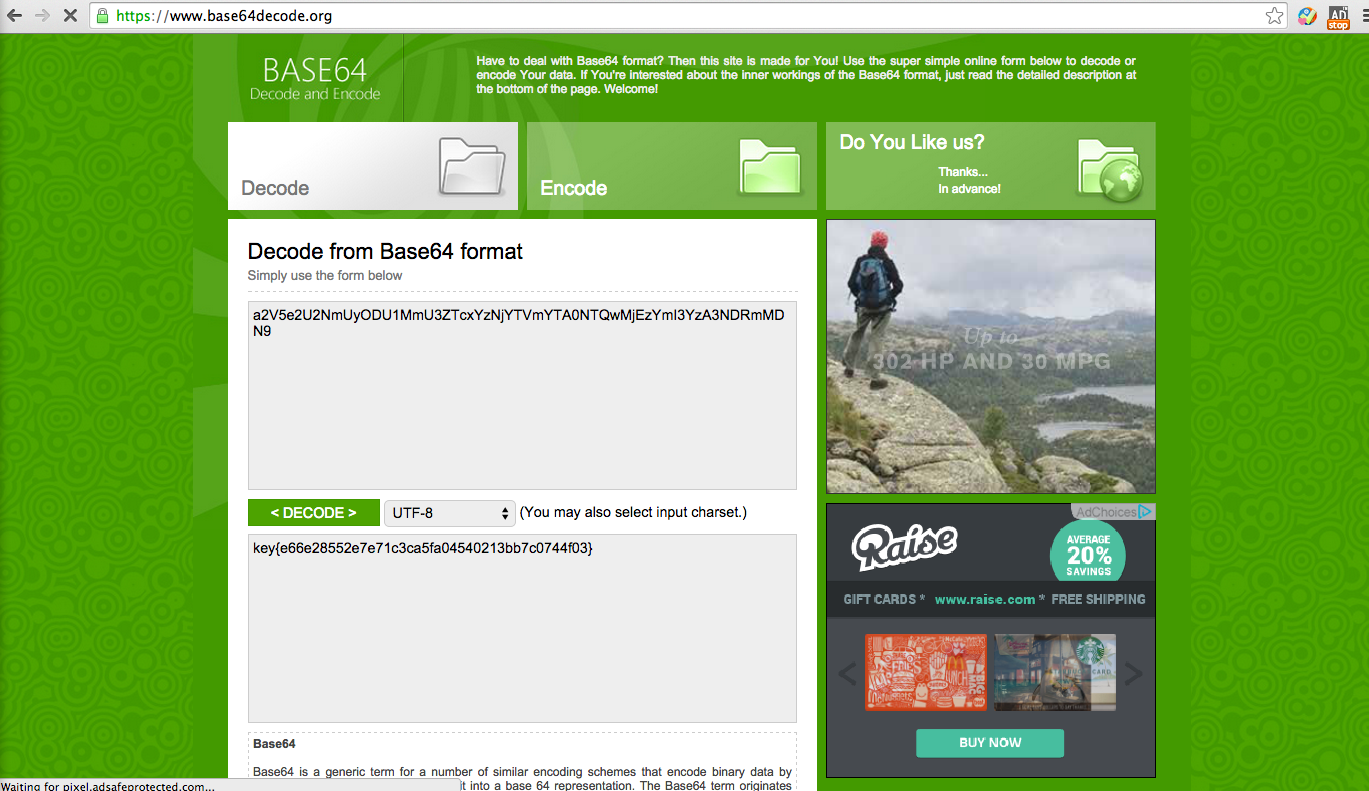
\includegraphics[scale=0.25]{images/flag9b} \\

\item \textbf{About my friend Karl (karl)...}: Brute-forcing WordPress passwords

\textbf{Location}: \texttt{http://67.23.79.113/wp-admin.php}

From the hint we surmised that 'karl' was a username for a login somewhere. 
Given that the board was part of a WordPress site, we guessed that it was for 
the site itself and we could break into the site administration page  
using 'karl' as the user. \\

From the WordPress login page, we started by randomly guessing some common 
dictionary words for the password, which proved unfruitful (and very tedious). 
Finally, we installed a FireFox plugin called 'FireForce', which, as the name 
implies, automatically brute-forces passwords for a given text input field. It
took FireForce just a few minutes to find karl's password and we were logged 
in. The flag itself was embedded in a private post: \\

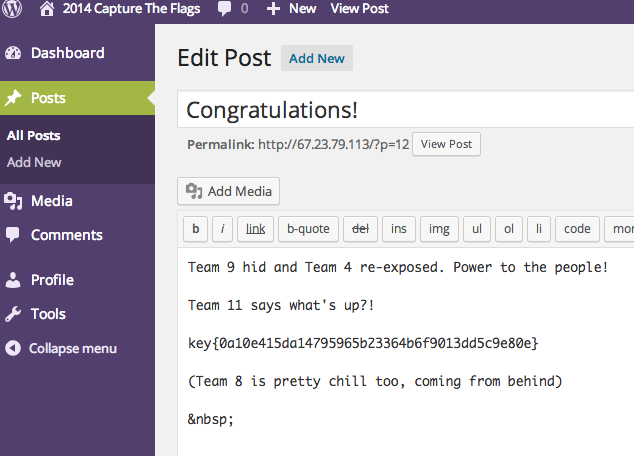
\includegraphics[scale=0.65]{images/flag10} \\

\newpage 

\item \textbf{Extra}:

We found the url \texttt{http://67.23.79.113/board.php?id=1} is vulnerable to SQL injection so we chose an SQL automation tool in Kali called SQLMAP to exploit the website database. We used the \texttt{--dbs} option to find out the names of the databases that exist on the website: \\

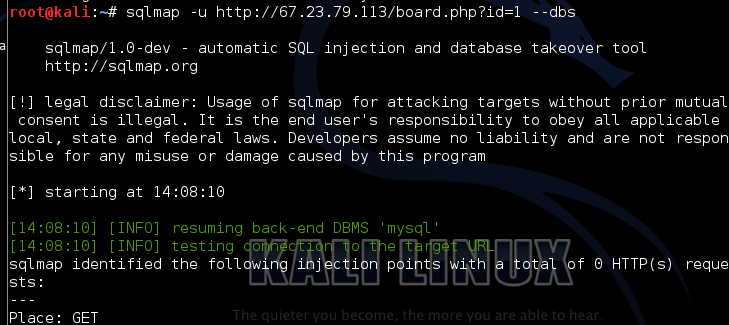
\includegraphics[scale=0.55]{images/flag8a} \\ \\

The output showed that there were five databases: \\

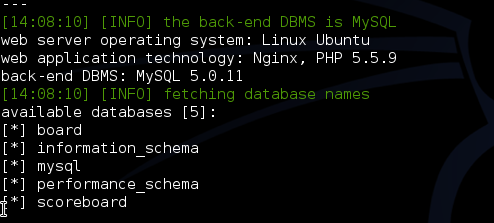
\includegraphics[scale=0.7]{images/flag8b} \\ \\

Wondering what tables existed in the 'scoreboard', we dumped the data out of it using \texttt{--dump} option: \\

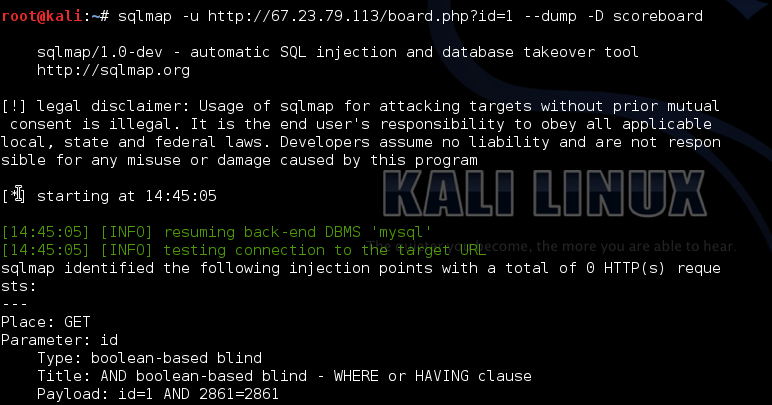
\includegraphics[scale=0.55]{images/extra1} \\ \\

Then we found this table in the output which contained all the flags that we had been looking for! \\

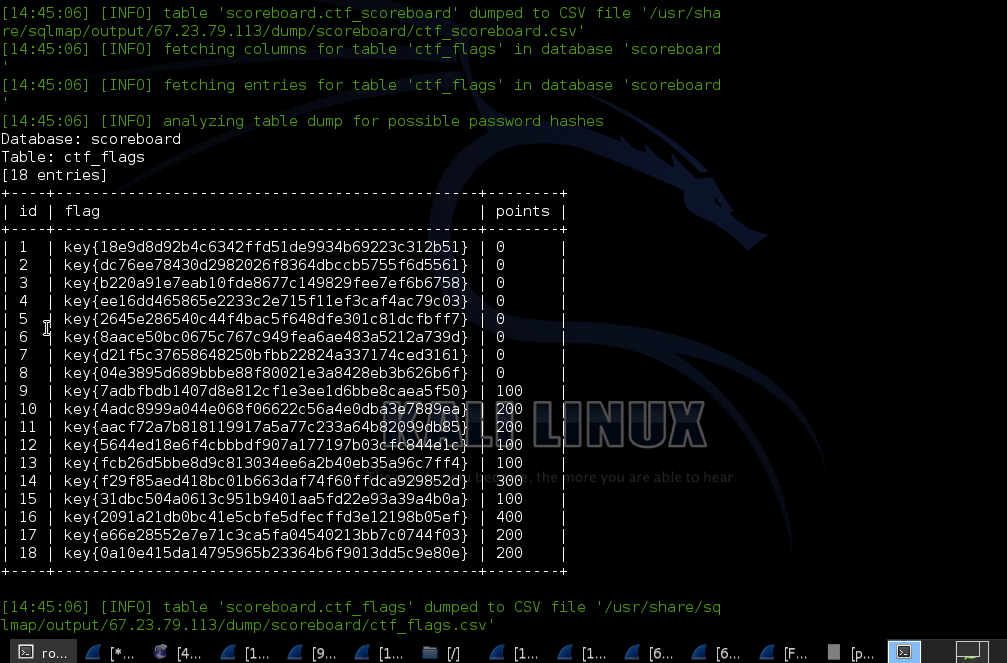
\includegraphics[scale=0.45]{images/extra2}

\end{enumerate}
\end{document}